\subsection{Ｃ\textsubscript{2}𝛑 Space}

\subsubsection{Fourier Basis $e^{ikt}$}

**$C_{2\pi}$  is a space of  continuous functions that is $2\pi$-periodic **. This is precisely the space of functions we are going to expand by fourier series. This chapter is dedicated to show that:

\begin{theorem}[  Space is Spanned by Fourier Basis]\textbf{$C_{2\pi}$}\\
$C_{2\pi}$ is an infinite-dimensional vector space spanned by $\{e^{ikt}\}_{k\in\mathbb{Z}}$. It is also an inner product space endorsed with the inner product:
\begin{equation}
\langle f,g \rangle = \frac{1}{2\pi}\int_{0}^{2\pi} fg^*dt
\end{equation}

\end{theorem}where $g^*$ denotes the \textit{complex conjugate} of $g$.

An elementary observation is that  $\{e^{ikt}\}_{k\in\mathbb{Z}}$ is orthonormal:

\begin{equation}
\frac{1}{2\pi}\int_0^{2\pi}e^{ik_1t}e^{-ik_2t}=\delta_{k_1k_2}
\end{equation}

\begin{proof}Since
\begin{equation}
\frac{1}{2\pi}\int_0^{2\pi}e^{ik_1t}e^{-ik_2t} &= \frac{1}{2\pi}\int_0^{2\pi}e^{i(k_1-k_2)t}
\end{equation}
\begin{equation}
\frac{1}{2\pi}\int_0^{2\pi}e^{i(k_1-k_2)t} = \frac{1}{2\pi}\int_0^{2\pi}\cos(k_1-k_2)t + i\sin(k_1-k_2)t
\end{equation}
If $k_1=k_2$ then it's clear we get 1. Otherwise, since both cosine and sine component above have period $\frac{2\pi}{k_1 -k_2}$ hence $2\pi$ is always a multiple:
\begin{equation}
\frac{1}{2\pi}\int_0^{2\pi}e^{i(k_1-k_2)t}=(k_1-k_2)\underbrace{\int_0^{2\pi}\cos(t)}_{0}+i(k_1-k_2)\underbrace{\int_0^{2\pi} \sin(t)}_{0}
\end{equation}

\end{proof}For arbitary $f:\mathbb{R}\to \mathbb{C}$, if we compute the representation using the infinite basis like what one would do in finite vector space, one would get:
\begin{equation}
\label{fe}
f=\sum_{k\in\mathbb{Z}}\langle f, \exp(ikt)\rangle \exp(ikt)
\end{equation}
This is known as the \textit{Fourier Series}.

\begin{framed}
\textbf{Infinite-dimensional Vector Space}\\
Note although (\ref{fe}) looks like the orthonormal basis expansion in finite-dimensional vector space, such expansion is not guaranteed to be valid by linear algebra theorems. In particular, we need to ensure (\ref{fe}) converges and it converges to $f$.
\end{framed}

So, in otherword, in order to shown we can do fourier expansion(that is, regarding $C_{2\pi}$ as an inner product space endorsed with the $L_2$ inner product), we would have to show its convergence for arbitrary $f\in C_{2\pi}$ first.

\subsubsection{Convergence of Fourier Series}

\paragraph{Theoretical Framework: The Overall Idea}

The overall theoretical framework is

\begin{framed}
\textbf{Big Idea}\\
First consider the infinity norm
\begin{equation}
\|f\|_{\infty}=\sup_t |f|
\end{equation}
Equip $C_{2\pi}$ with the iniftity norm to obtain the Banach Space $(C_{2\pi}, \|\cdot\|_{\infty})$  \footnote{A Banach space is a normed complete vector space}. Then show a weaker form of convergence -- \textbf{Convergence in Abel's Sense} in the Banach space. Finally, since different norms essentially agree with each other, we note that Hilbert Space$(C_{2\pi}, \langle\cdot, \cdot, \rangle_{2})$ inherits the same sense of convergence. This justifies fourier expansion:
\begin{equation}
f=\sum_{k\in\mathbb{Z}}\langle f, \exp(ikt)\rangle \exp(ikt)
\end{equation}

\begin{figure}[!htbp]
\centering
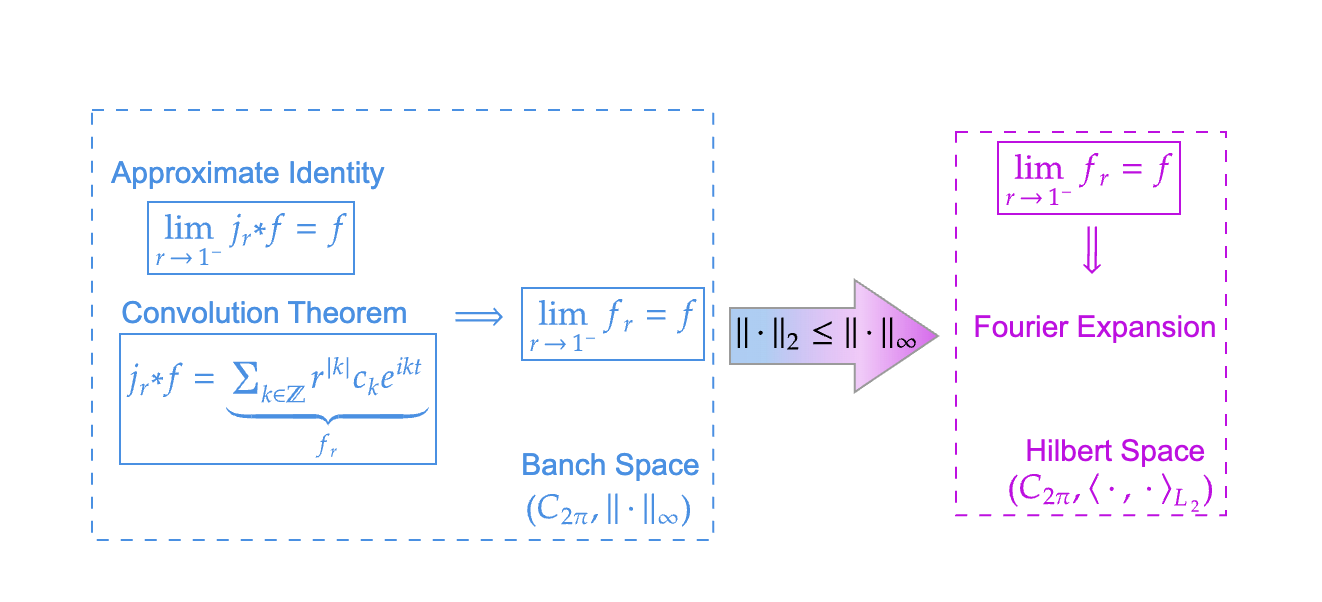
\includegraphics[width=0.7\linewidth]{files/convergence_of_fouri-3fbfbe8d21f6e4000ab45bb3f05154bc.png}
\end{figure}
\end{framed}

\paragraph{Convergence in Abel's Sense}

\begin{figure}[!htbp]
\centering
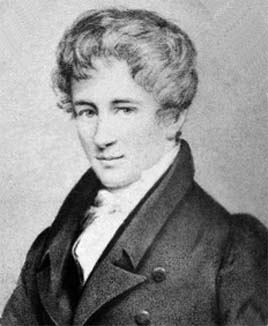
\includegraphics[width=0.7\linewidth]{files/Niels_Henrik_Abel-c40d66306f3721b227d2dd8e2dcabb34.jpg}
\caption*{The famous Norwegian Mathematician Niels Henrik Abel. Quite a good-looking fella ei? Probably everyone's first encoutner would be \textbf{Abel's test} from Calculus, i.e. if $\sum_k a_k$ is convergent, then $\sum_k a_kb_k$ is convergent iff $b_k$ is \textit{monotone} and \textit{bounded}.}
\end{figure}

\begin{definition}[Abel Summation]Consider a constant-valued series $\sum_k a_k$, the corresponding Abel's summation transform it into a power series $\sum_k a_k r^k$. We say $\sum_k a_k$ converges to to $c$ \textit{in the Abel's sense} if
\begin{equation}
\lim_{r \to 1^-}\sum_{k=1}^{\infty} a_k r^k = c
\end{equation}
where $r\to 1^ -$ denotes left limit.

\end{definition}\textit{Rmk. Normal convergence implies Abel's convergence}

\begin{proof}[Normal convergence implies Abel’s convergence ⏩]\textbf{Want}: $\forall \epsilon >0$, $\exists \delta >0$
s.t. $\forall r > 1 -\delta$ we have $\left|\lim_{k\to \infty}\sum_{j=1}^k a_jr^j - c\right|<\epsilon$.

Denote the partial sum as:
\begin{equation}
s_k :=\sum_{j=1}^k a_j
\end{equation}

The goal is to use $\delta$ to control the following quanitity
\begin{equation}
E:=\left|\lim_{k\to \infty}s_j - c\right|
\end{equation}

To do so, we would like to utillize the fact the series is convergent. One way to do so is  manipulate the quantity such that $s_j -c$ appears somewhere:
\begin{equation}
\left|\lim_{k\to \infty}s_j - c\right| &= \left|\lim_{k\to \infty}\sum_{j=1}^k (\textcolor{orchid}{s_j}-\textcolor{pink}{s_{j-1}})r^j - c\right| \\
&= 
\left|\textcolor{orchid}{\lim_{k\to \infty}\sum_{j=1}^k s_jr^j} -  \textcolor{pink}{\lim_{k\to \infty}\sum_{j=1}^{k-1} s_jr^{j+1}} - c\right| \\
&= 
\left| \lim_{k\to\infty}\left[\textcolor{orchid}{s_kr^k} + (\textcolor{orchid}{1}-\textcolor{pink}{r})\sum_{j=1}^{k-1}s_jr^j\right]-c\right|
\end{equation}
Note that

\begin{enumerate}
\item $\lim_{k\to \infty}s_kr^k = 0$ since we know $\lim_{k\to \infty}s_k$ exists and for $|r|<1$, we have $\lim_{k\to\infty}{r^k}=0$ hence by standard limit product law we have

\begin{equation}
\lim_{k\to \infty}s_kr^k=\lim_{k\to \infty}s_k\lim_{k\to \infty}r^k=0
\end{equation}


\item We can write $c$ akin to the form of the term $(\textcolor{orchid}{1} -\textcolor{pink}{r})\sum_{j=1}^{k -1}s_jr^j$, i.e.

\begin{equation}
c=(1-r)\frac{c}{1-r}=(1-r)\lim_{k\to\infty}\sum_{j=1}^k cr^j
\end{equation}
\end{enumerate}

Hence the quantity we want to control becomes:
\begin{equation}
E=\left| (1-r)\sum_{j=1}^{\infty} (s_j-c)r^j\right|
\end{equation}
Intuitively, for small $j$, $s_j -c$ can be large but then we can make the quantity small by picking sufficiently small $\delta=1 -r$. On the otherhand, as the series converge, the tail terms $(s_j -c)$ can be arbitraily small by definition. To convey such idea mathematically, we use a common technique which is to split the series and control the leading and the tail sum respectively:
\begin{equation}
E &= \left| (1-r)\sum_{j=1}^{N} (s_j-c)r^j + (1-r)\sum_{j=N+1}^{\infty} (s_j-c)r^j\right| \\
&\leq \left| (1-r)\sum_{j=1}^{N} (s_j-c)r^j \right| +  \left|(1-r)\sum_{j=N+1}^{\infty} (s_j-c)r^j\right| \\
&\leq  (1-r)\sum_{j=1}^{N} |s_j-c|r^j  +  (1-r)\sum_{j=N+1}^{\infty} |s_j-c|r^j
\end{equation}

\begin{enumerate}
\item For the tail sum, we notice that, by the convergence of the sequence $s_j$, we can pick an $N$ such that $\forall j > N$, $|s_j -c|<\epsilon/2$. Hence:

\begin{equation}
(1-r)\sum_{j=N+1}^{\infty} |s_j-c|r^j &\leq \frac{\epsilon}{2}(1-r)\sum_{j=N+1}^{\infty} r^j \\ 
&= \frac{\epsilon}{2}
\end{equation}


\item For the leading sum, we would like to control:

\begin{equation}
(1-r)\sum_{j=1}^{N} |s_j-c|r^j&\leq \epsilon/2 \\
\end{equation}


if we let $M:=(1 -r)\sum_{j=1}^{N} |s_j -c|$, then $\sum_{j=1}^{N} |s_j -c|r^j \leq M$, then:

\begin{equation}
(1-r)\sum_{j=1}^{N} |s_j-c|r^j\leq (1-r)M = \delta M
\end{equation}


Hence we obtained the requirement on $\delta$:

\begin{equation}
\delta \leq \frac{\epsilon}{2M}
\end{equation}


As desired.
\end{enumerate}

\end{proof}\paragraph{Algebra}

Recall that we can construct vector space(denoted $V$) from fields(denoted by $\mathbb{F}$) by stacking elements from the field together. Valid operators include addition of vector and scalar multiplications. \textit{Algebra} takes one more step and introduce ``vector-vector'' multiplications:

\begin{definition}[Algebra]An \textbf{algebra} is a vector space equipped with a binary operatation $V\times V\to V$ that is \textit{commutative}, \textit{associative} and \textit{distributive}.

\end{definition}In this section, we show that the infinite dimensional vector space $C_{2\pi}$ spanned by $\{e^{ik\pi}\}_{k\in\mathbb{Z}}$ equipped with convolution